
\begin{figure}[ht]
  \centering
  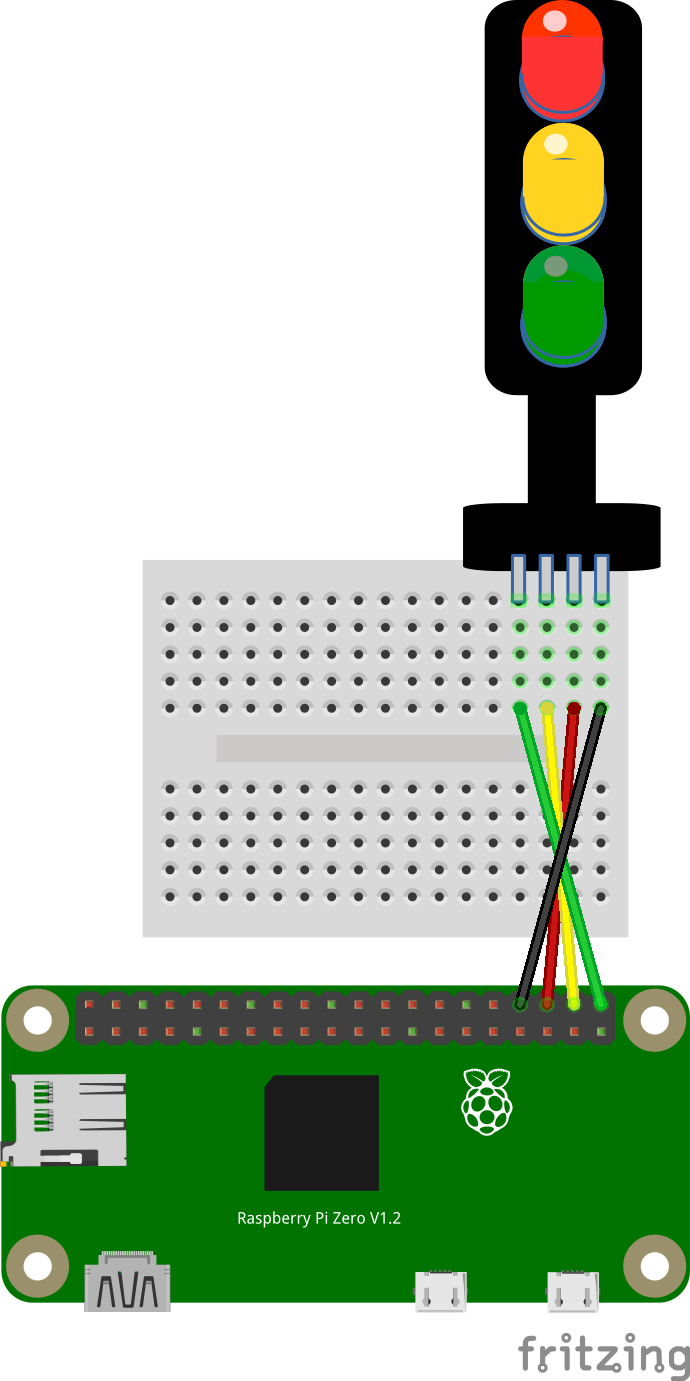
\includegraphics[scale=0.25, angle=-90]{images/TrafficLight_Steckplatine.png}	
  %	\caption{}
  \label{LED_Steckplatine}
\end{figure}

%\begin{figure}[ht]
%	\centering
%	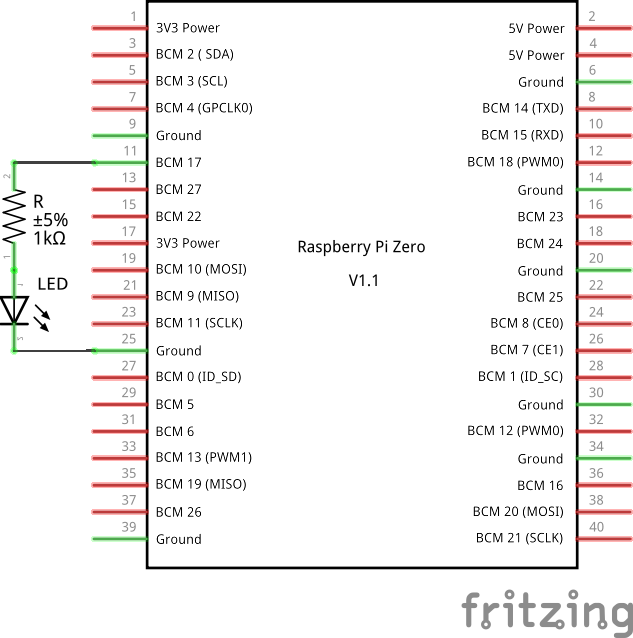
\includegraphics[scale=0.25]{images/LED_Schaltplan.png}	
%	%	\caption{}
%	\label{LED_Schaltplan}
%\end{figure}

\subsection{Shell}

%\begin{console}
%	gpio -g mode 17 out
%	gpio -g write 17 1
%	gpio -g write 17 0
%	gpio -g mode 17 in
%\end{console}

%https://de.scribd.com/doc/101830961/GPIO-Pads-Control2

% gpio drive 0 0  2 mA
% gpio drive 0 3  8 mA <- default
% gpio drive 0 7  16 mA


\subsection{C\#}

\subsection{C}

\begin{console}
	geany &
\end{console}

Nun kann man ein neues Projekt erstellen, dazu w�hlt man \texttt{Projekt} $\rightarrow$ \texttt{Neu...}. Dann Gibt man den Namen des Projekts an. Das Anlegen der Verzeichnisse muss man auch noch best�tigen. 

%\begin{figure}[ht]
%	\centering
%	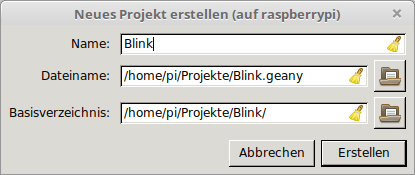
\includegraphics[scale=0.48]{images/Geany_Projekt.png}
%	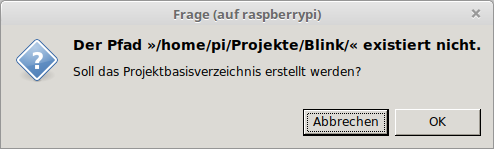
\includegraphics[scale=0.42]{images/Geany_Projekt2.png}
%%	\caption{}
%	\label{Geany-create}
%\end{figure}

Danach w�hlt man \texttt{Datei} $\rightarrow$ \texttt{Speichern unter} um die unbenannte Datei mit dem Namen "`TrafficLight.c"' speichern zu k�nnen. Nun kann man den folgenden C-Source eingeben.

\lstset{language=C, caption=, label=TrafficLightProgram, frame=single, basicstyle=\ttfamily
	\footnotesize, breakatwhitespace=false, showstringspaces=false, showtabs=false, tabsize=2 }
\lstinputlisting{source/TrafficLight.c}

Jetzt darf man nicht vergessen im Men� unter \texttt{Erstellen} $\rightarrow$ \texttt{Kommandos zum Erstellen konfigurieren} die Wiring Pi Library mit "`-lwiringPi"' bei Compile und Build zu erg�nzen.

\begin{figure}[ht]
	\centering
	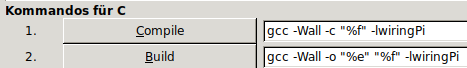
\includegraphics[scale=0.48]{images/Geany_Create_Wiringpi.png}
	%	\caption{}
	\label{Geany-create}
\end{figure}

Nun kann man das Projekt mit den Ziegel-Icon 
\includegraphics[scale=0.4]{images/Geany_Icon_Erstellen.png} erstellen bzw. kompilieren und danach mit dem Zahnrad-Icon 
\includegraphics[scale=0.4]{images/Geany_Icon_Ausfuehren.png}  ausf�hren.  

\subsection{Python}
Um das Python Programm auszuf�hren muss man eine neue Datei anlegen und 
unter \texttt{Datei} $\rightarrow$ \texttt{Speichern unter} die
Datei mit dem Namen "`TrafficLight.py"' abspeichern. Anschlie�end kann man
folgenden Python-Source einf�gen:

\lstset{language=Python, caption=, 
        label=LEDProgram, frame=single, basicstyle=\ttfamily
	      \footnotesize, breakatwhitespace=false, showstringspaces=false, 
        showtabs=false, tabsize=2 }
\lstinputlisting{source/TrafficLight.py}

Anschlie�end kann man das Programm mit dem Zahnrad-Icon

\includegraphics[scale=0.4]{images/Geany_Icon_Ausfuehren.png}  ausf�hren.  
